\documentclass[smaller]{beamer}
\usetheme{Madrid}
\usecolortheme{default}
% Replace with the burgundy/maroon color from the image
\definecolor{headercolor}{RGB}{188,39,50}
\setbeamercolor{palette primary}{bg=headercolor,fg=white}
\setbeamercolor{palette secondary}{bg=headercolor,fg=white}
\setbeamercolor{palette tertiary}{bg=headercolor,fg=white}
\setbeamercolor{palette quaternary}{bg=headercolor,fg=white}
\setbeamercolor{structure}{fg=headercolor}
\usepackage{graphicx}
\usepackage{amsmath}

% Adjust bullet appearance
\setbeamertemplate{itemize item}{\usebeamercolor[fg]{structure}\large\textbullet}

\title{A Robust Nonparametric Framework for \\Repeated Spatial Clustering}
\subtitle{Insights from Cell Types in Spatial Omics}
\author{Mithun Manivannan}
\date{May 14-16, 2024}

\begin{document}

% Slide 1 - Title
\begin{frame}
\titlepage
\end{frame}

% Slide 2 - Problem & Method
\begin{frame}{The Challenge in Spatial Clustering}

% Two figures at the top - Updated to two separate figures
\begin{figure}
\centering
\begin{minipage}{0.43\textwidth}
\centering
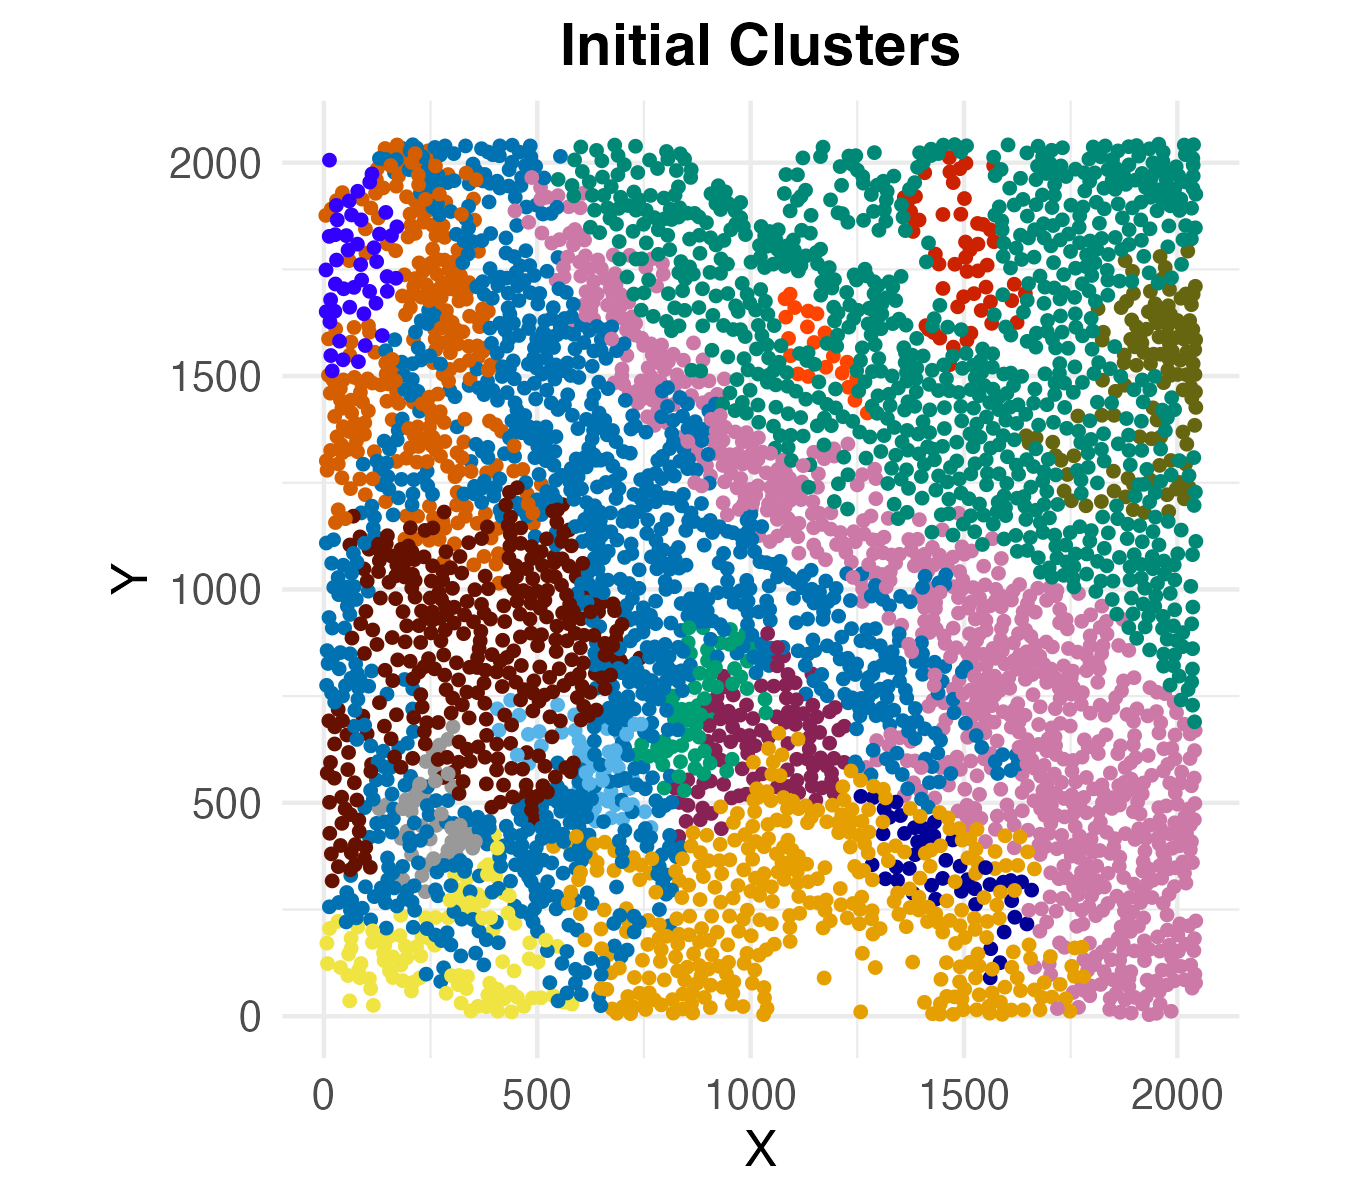
\includegraphics[width=\textwidth]{initial_clusters_plot.png} % Use the new initial clusters plot
\end{minipage}
\hfill % Space between figures
\begin{minipage}{0.43\textwidth}
\centering
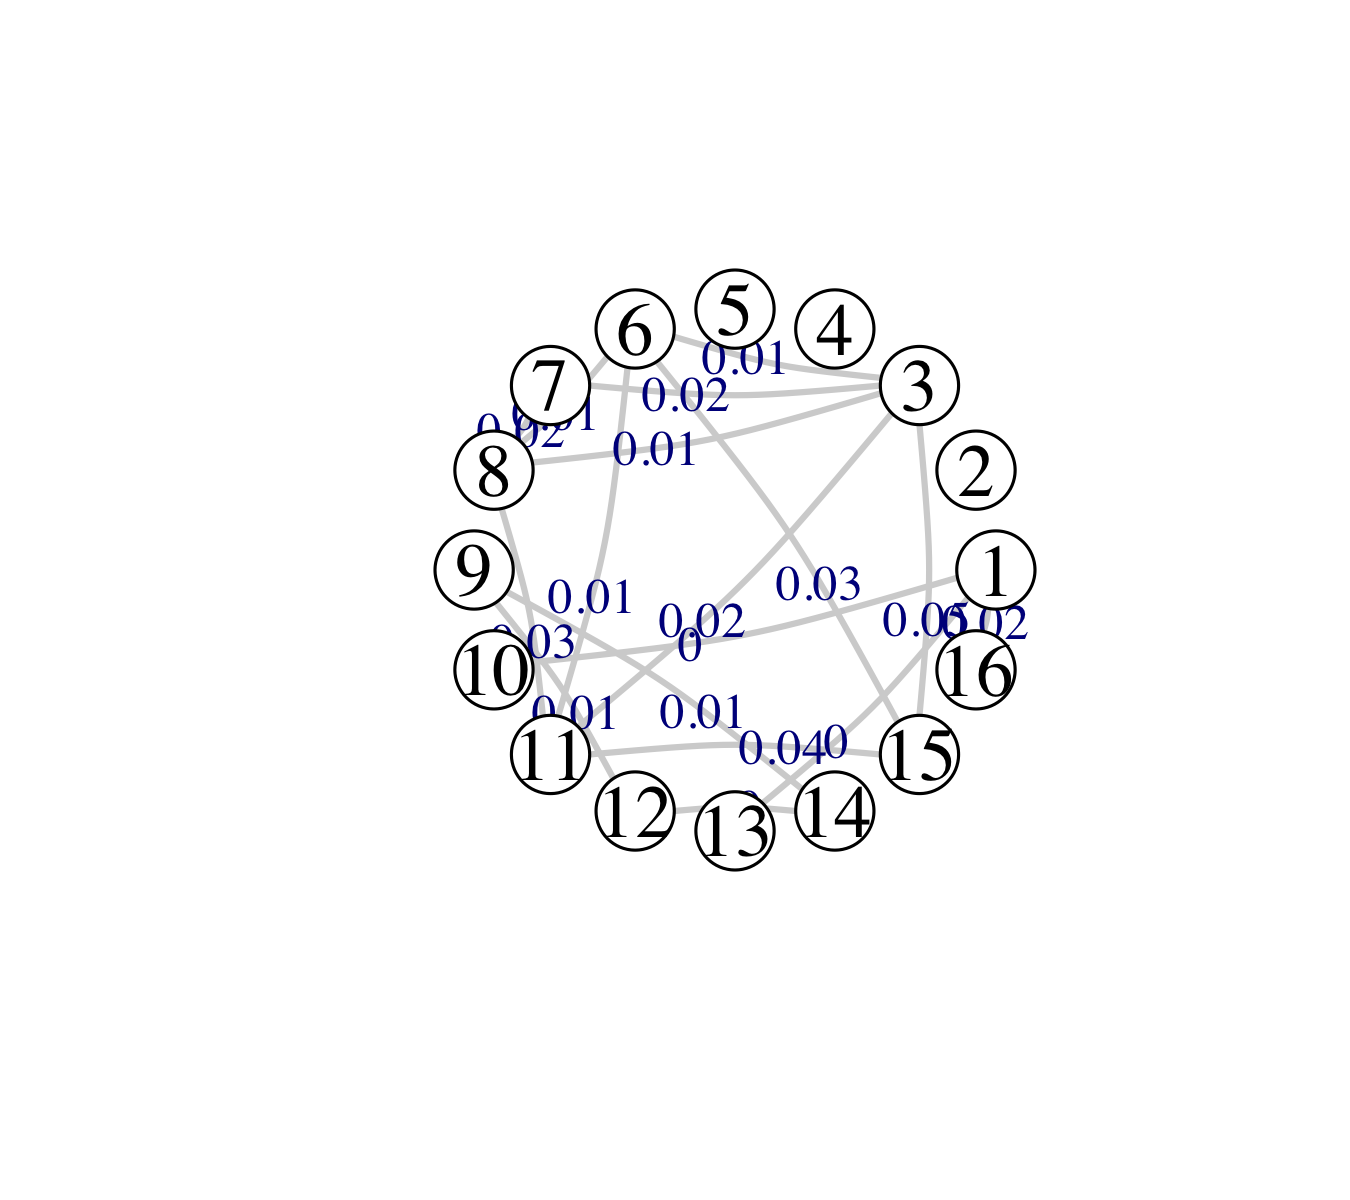
\includegraphics[width=\textwidth]{similarity_graph.png} % Use the new similarity graph
\end{minipage}
\end{figure}

\small\textbf{Current Methods' Limitations:}
\begin{itemize}
\setlength{\itemsep}{0em} % Reduced item separation to minimum
    \item Attribute-only methods lose spatial contiguity
    \item Current methods cannot capture repeated spatial patterns
    \item Methods assume Markov random field for attributes
    \item Critical for tumor microenvironment analysis
\end{itemize}

\small\textbf{Our Solution:}
\begin{itemize}
\setlength{\itemsep}{0em} % Reduced item separation to minimum
    \item Two-step framework: Constrained hierarchical clustering \& MMD test w/ block permutation
    \item Preserves spatial structure while detecting similarity
\end{itemize}

\end{frame}

% Slide 3 - Results
\begin{frame}{Detecting Repeated Tumor Microenvironments}

% Two figures at the top - Updated to single combined figure
\begin{figure}
\centering
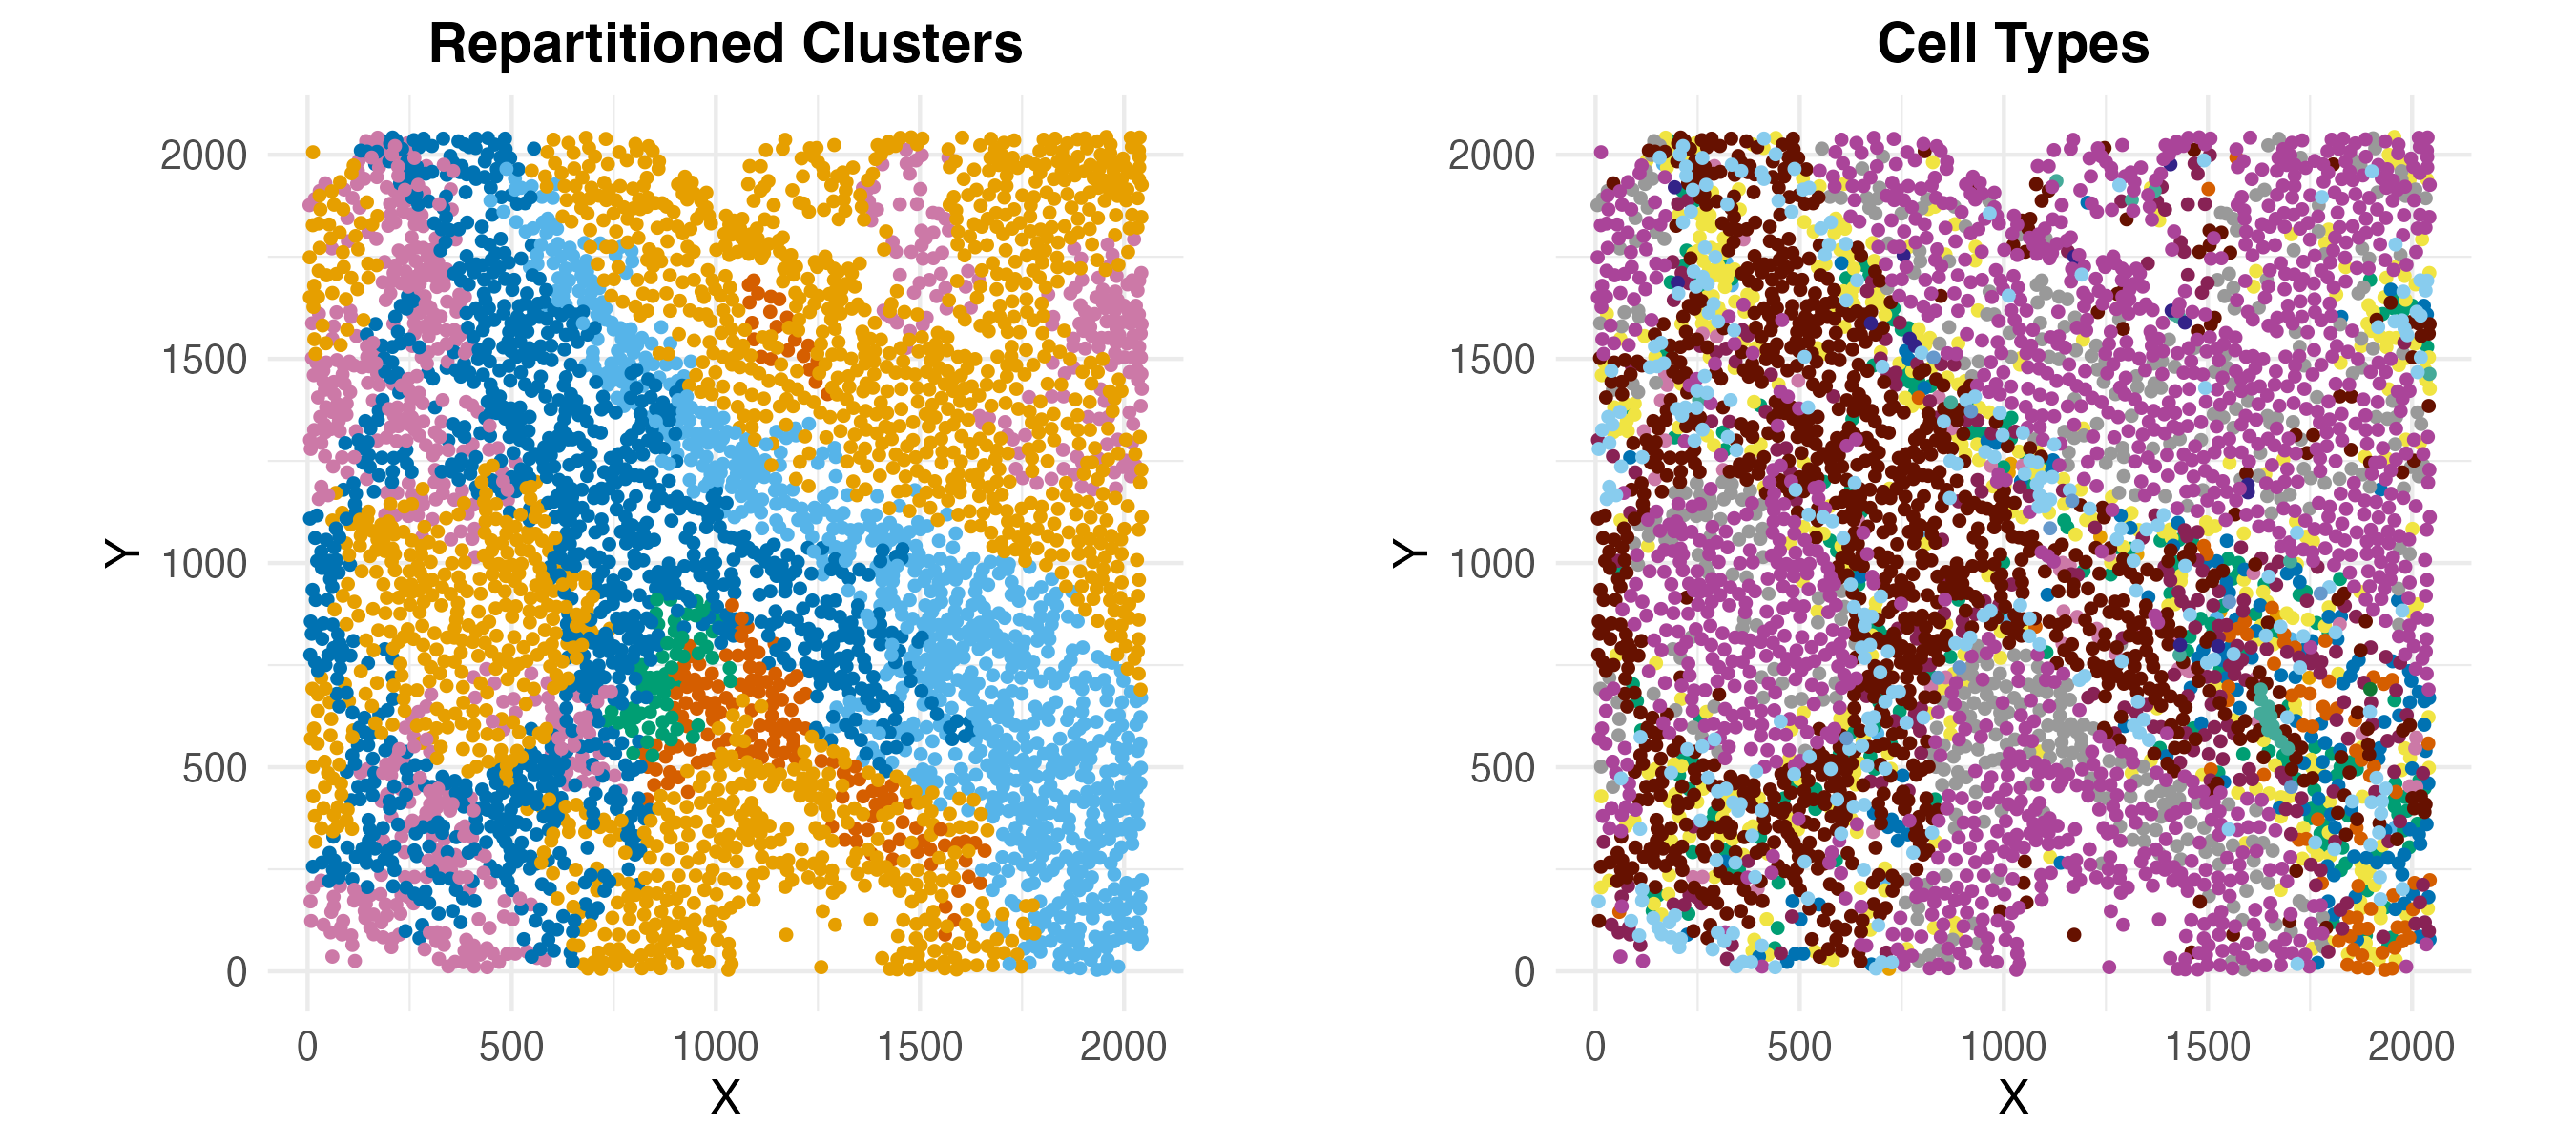
\includegraphics[width=0.80\textwidth]{figure_slide3.png} % Use the combined figure for slide 3 - Further Reduced width
\end{figure}

\small\textbf{Application to TNBC Data:}
\begin{itemize}
\setlength{\itemsep}{0em} % Reduced item separation to minimum
    \item Triple-negative breast cancer samples
    \item 16 cell types (binary features)
    \item Identified functionally similar tumor regions
\end{itemize}

\small\textbf{Impact:}
\begin{itemize}
\setlength{\itemsep}{0em} % Reduced item separation to minimum
    \item More accurate tumor classification
    \item Better understanding of cancer heterogeneity
    \item Adaptable to diverse spatial data
\end{itemize}

\end{frame}

\end{document}